\documentclass[11pt,a4paper]{article}

\usepackage[utf8]{inputenc}
\usepackage[margin=2.5cm]{geometry}
\usepackage{amsmath,amssymb,amsfonts}
\usepackage{booktabs,tabularx,multirow}
\usepackage{algorithm}
\usepackage{algpseudocode}
\usepackage{xcolor}
\usepackage{tikz}
\usetikzlibrary{shapes.geometric,arrows.meta,positioning,calc,fit,backgrounds}
\usepackage{fancyhdr}
\usepackage{microtype}
\usepackage[colorlinks=true,linkcolor=blue!70!black,citecolor=blue!70!black,urlcolor=blue!70!black]{hyperref}

% Header and Footer setup conforming to Patent Specification Standards
\pagestyle{fancy}
\fancyhf{}
\lhead{\footnotesize \textbf{PATENT SPECIFICATION} | APPLICATION NO.: IP-2026-ENG-8402}
\rhead{\footnotesize \textbf{SHEET \thepage\ OF \pageref{LastPage}}}
\lfoot{\footnotesize CONSTRUMINDNET: SPATIO-TEMPORAL EQUIPMENT ALLOCATION}
\rfoot{\footnotesize APPLICANTS: SUDHA ET AL.}
\cfoot{}
\renewcommand{\headrulewidth}{0.6pt}
\renewcommand{\footrulewidth}{0.4pt}

\setlength{\parindent}{0pt}
\setlength{\parskip}{0.8em}

\begin{document}

% -----------------------------------------------------------------------------
% FORM 2 - PATENT TITLE & APPLICATION COVER
% -----------------------------------------------------------------------------
\begin{center}
    {\large \textbf{FORM 2}}\\[0.3em]
    {\large \textbf{THE PATENTS ACT, 1970 (39 OF 1970)}}\\[0.2em]
    {\normalsize \textbf{\& THE PATENTS RULES, 2003}}\\[0.5em]
    {\large \textbf{COMPLETE SPECIFICATION}}\\[0.2em]
    {\small (See section 10 and rule 13)}
\end{center}

\vspace{1em}
\noindent\rule{\textwidth}{1.2pt}
\vspace{0.5em}

\begin{center}
    {\Large \textbf{A HYBRID SPATIO-TEMPORAL DEEP LEARNING SYSTEM AND METHOD FOR MULTI-HORIZON HEAVY EQUIPMENT ALLOCATION AND FLEET SCHEDULING}}
\end{center}

\vspace{0.5em}
\noindent\rule{\textwidth}{1.2pt}
\vspace{1em}

\textbf{APPLICANTS AND INVENTORS:}
\begin{enumerate}
    \item \textbf{Dr. Danthuluri Sudha}, Indian National, Department of Computer Science and Technology, Dayananda Sagar University, Devarakaggalahalli, Harohalli, Kanakapura Road, Bangalore, Karnataka, India - 562112.
    \item \textbf{Dr. Santosh Kumar Jankatti}, Indian National, Department of Computer Science and Technology, Dayananda Sagar University, Bangalore, Karnataka, India - 562112.
    \item \textbf{Dr. Ramandeep Kaur}, Indian National, Department of Computer Science and Technology, Dayananda Sagar University, Bangalore, Karnataka, India - 562112.
    \item \textbf{Dr. Bondu Venkateswarlu}, Indian National, Department of Computer Science and Engineering, Dayananda Sagar University, Bangalore, Karnataka, India - 562112.
    \item \textbf{Dr. T. Gayathri}, Indian National, Department of Computer Science and Engineering, Dayananda Sagar University, Bangalore, Karnataka, India - 562112.
    \item \textbf{Dr. G. Manjula}, Indian National, Department of Computer Science and Design, Dayananda Sagar Academy of Technology and Management, Bangalore, Karnataka, India - 560082.
    \item \textbf{Dr. Harish H. Kenchannavar}, Indian National, Department of Computer Science and Engineering (Data Science), Dayananda Sagar College of Engineering, Bangalore, Karnataka, India - 560078.
\end{enumerate}

\vspace{1em}
\textbf{PREAMBLE TO THE DESCRIPTION:}\\
\textit{The following specification particularly describes the invention and the manner in which it is to be performed.}

\newpage

% -----------------------------------------------------------------------------
% COMPLETE SPECIFICATION BODY
% -----------------------------------------------------------------------------

\section{FIELD OF THE INVENTION}
\noindent The present invention relates generally to the technical fields of artificial intelligence, spatio-temporal deep learning, and industrial telematics. More specifically, the present invention relates to an automated, intelligent, and constraint-aware system and computer-implemented method for multi-horizon heavy equipment allocation, fleet dispatching, and dynamic maintenance scheduling across distributed, multi-site civil infrastructure and industrial construction projects.

\section{BACKGROUND OF THE INVENTION AND PRIOR ART}
\noindent In contemporary civil infrastructure engineering, commercial construction, and regional megaprojects, heavy mobile and static industrial machinery---including hydraulic excavators, dump trucks, heavy mobile cranes, tower cranes, concrete boom pumps, transit mixers, motor graders, compaction rollers, bulldozers, and deep foundation piling rigs---constitute immense capital expenditure assets. Operational efficiency, contract adherence, project delivery velocity, and operational carbon footprints depend heavily on the optimal temporal allocation and spatial dispatching of these assets across geographically dispersed project sites and central maintenance depots.

\noindent In real-world enterprise operations, fleet dispatching requires continuous coordination between heterogeneous machine specifications (e.g., engine operating hours, load capacities, boom reaches, fuel consumption rates, mechanical ages) and time-varying site requirements across multiple sequential construction phases (e.g., Earthworks, Foundation Piling, Superstructure Logistics, Facade Installation, and MEP Finishing). Inefficiencies in equipment scheduling cause severe project disruptions: idle machinery depreciation, unscheduled breakdown propagation, bottlenecking on critical-path milestones, excessive transit mobilization mileage, and cascading contractual financial penalties.

\noindent Conventional equipment scheduling systems predominantly rely on classical Operations Research (OR) methodologies, notably Mixed-Integer Linear Programming (MILP), Branch-and-Bound algorithms, or greedy heuristic dispatching rules (e.g., Earliest Due Date [EDD], First-Come-First-Served [FCFS], and Nearest-Neighbor heuristics). While MILP formulations offer theoretical optimality under deterministic assumptions, they suffer from combinatorial explosion ($NP$-hard computational complexity), rendering them intractable for real-time dispatching across enterprise fleet sizes ($>40$ machines) over multi-week planning horizons. Furthermore, greedy heuristic rules make myopic local choices that fail to account for downstream phase handovers, resulting in severe schedule slippage and frequent machine re-dispatching churn.

\noindent More recently, sequential deep learning models, such as Recurrent Neural Networks (RNNs), Long Short-Term Memory networks (LSTMs), and self-attention Transformers, have been investigated for time-series forecasting in industrial logistics. However, existing deep learning approaches suffer from several acute technical drawbacks:
\begin{enumerate}
    \item \textbf{Multi-Horizon Rollout Error Drift:} Purely data-driven sequence networks suffer from rapid error compounding when deployed in multi-step autoregressive rollouts, leading to catastrophic allocation drift over extended horizons.
    \item \textbf{Neglect of Non-Euclidean Logistics Graphs:} Standard neural networks assume regular Euclidean coordinates, failing to represent real-world road networks, transit tolls, mobilization travel durations, and shared maintenance depot constraints.
    \item \textbf{Lack of Operational Constraint Enforcement:} Unconstrained neural networks frequently output schedules that violate hard physical and contractual boundaries, such as scheduling machinery during active preventive maintenance work orders or exceeding site parking capacities.
    \item \textbf{Poor Cross-Project Generalization:} Neural models trained on mature commercial building projects experience severe distribution shifts when transferred to newly initiated infrastructure or highway projects.
\end{enumerate}

\noindent Therefore, there exists an urgent, unfulfilled technological need in the construction and fleet management industries for an intelligent, constraint-aware, hybrid spatio-temporal deep learning system and method that overcomes the computational intractability of classical mathematical solvers while eliminating the cumulative error drift and constraint violations of unconstrained neural models.

\section{OBJECTS OF THE INVENTION}
\noindent The primary object of the present invention is to provide an end-to-end hybrid spatio-temporal deep learning system and method (termed \textbf{ConstrumindNet}) for multi-horizon heavy equipment allocation and fleet scheduling across geographically distributed construction project sites.

\noindent Another object of the present invention is to provide a multi-scale temporal learning hierarchy that simultaneously models high-frequency daily operational shifts, medium-term construction phase transitions, and long-term project lifecycle horizons, thereby suppressing multi-step cumulative rollout drift.

\noindent Yet another object of the present invention is to provide a spatial Graph Attention Network (GAT) that models non-Euclidean road logistics networks, transit distances, mobilization costs, and regional site-depot teleconnections.

\noindent Still another object of the present invention is to provide a Latent Feature Refinement (LFR) module that compresses high-dimensional latent states into a compact bottleneck representation and executes expressive nonlinear feature-mixing transformations to capture high-order machinery-project synergies.

\noindent A further object of the present invention is to provide an operational-aware physics and consistency regularisation engine that penalizes maintenance schedule collisions, suppresses unnecessary inter-site mobilization churn, and aligns latent representations across heterogeneous project regimes.

\noindent An additional object of the present invention is to provide a real-time decision engine capable of generating conflict-free, multi-horizon equipment allocations with sub-second inference latency ($<0.5$ seconds), enabling instantaneous re-dispatching during unexpected site breakdowns.

\section{SUMMARY OF THE INVENTION}
\noindent The present invention discloses an automated, computer-implemented hybrid spatio-temporal deep learning system and method for multi-horizon heavy equipment allocation and fleet scheduling. 

\noindent According to a first aspect of the present invention, the system comprises:
\begin{enumerate}
    \item A \textbf{Telematics and Schedule Ingestion Module} configured to receive and temporally synchronize continuous CAN-bus fleet telemetry data, multi-project construction phase schedules, workshop maintenance work orders, and geographic information system (GIS) transit distance matrices into a unified spatio-temporal state tensor $X_t \in \mathbb{R}^{N_s \times N_e \times C}$, where $N_s$ denotes spatial locations (project sites and central depots), $N_e$ denotes the fleet size, and $C$ denotes operational feature channels;
    \item A \textbf{Spatial Graph Attention Network (GAT) Subsystem} configured to represent the distributed construction sites and depots as a non-Euclidean weighted directed graph $\mathcal{G} = (\mathcal{V}, \mathcal{E}_g, \mathcal{W})$, computing learned spatial attention coefficients across road transit corridors;
    \item A \textbf{Multi-Scale Temporal Transformer Encoder} configured to hierarchically process sliding historical context windows of length $L$ across tactical daily shifts (1--3 days), phase handovers (7--14 days), and strategic milestones (30+ days), generating a spatio-temporal latent representation $Z \in \mathbb{R}^{N \times d}$;
    \item A \textbf{Latent Feature Refinement (LFR) Module} configured to project the latent representation $Z$ into a lower-dimensional bottleneck space $Z_c \in \mathbb{R}^{N \times q}$ ($q \ll d$), subject the compressed tokens to multi-stage nonlinear feature-mixing transformations, and project refined features back to embedding space via a trainable residual gating mechanism $Z^* = Z + \alpha Z_r$;
    \item A \textbf{Multi-Horizon Forecast Decoder} configured to simultaneously predict point estimates and allocation state fields $\widehat{X}_{t+1:t+H}$ across all future lead times $h \in \{1, 2, \dots, H\}$ in a direct multi-step mapping; and
    \item An \textbf{Operational-Aware Regularisation Engine} configured to optimize model parameters via a composite loss function comprising a task prediction loss, a maintenance-schedule collision penalty ($\mathcal{L}_{\text{maint}}$), a mobilization transit distance penalty ($\mathcal{L}_{\text{transit}}$), and a cross-regime Maximum Mean Discrepancy (MMD) distribution alignment loss ($\mathcal{L}_{\text{regime}}$).
\end{enumerate}

\noindent According to a second aspect of the present invention, there is provided a computer-implemented method executed by the system for generating stable, conflict-free multi-horizon equipment allocations, dynamically auditing schedules against active maintenance work orders, and executing sub-second dispatching adjustments upon equipment failure.

\section{BRIEF DESCRIPTION OF THE ACCOMPANYING DRAWINGS}
\noindent The technical features and advantages of the present invention will become more apparent from the following detailed description taken in conjunction with the accompanying drawings, in which:

\begin{itemize}
    \item \textbf{FIG. 1} illustrates an overall system architectural block diagram of the intelligent spatio-temporal equipment allocation and fleet scheduling system (\textbf{ConstrumindNet}), in accordance with an exemplary embodiment of the present invention;
    \item \textbf{FIG. 2} illustrates a schematic network diagram of the non-Euclidean spatial logistics graph interconnecting project sites and central maintenance depots across an urban-regional corridor;
    \item \textbf{FIG. 3} illustrates a detailed block diagram of the Latent Feature Refinement (LFR) module and residual gated fusion pathway;
    \item \textbf{FIG. 4} illustrates a workflow diagram of the multi-scale temporal decomposition hierarchy modeling daily shifts, phase handovers, and project lifecycles;
    \item \textbf{FIG. 5} illustrates a flowchart of the computer-implemented end-to-end training procedure integrating operational-aware regularisation constraints; and
    \item \textbf{FIG. 6} illustrates a flowchart of the dynamic real-time multi-horizon rollout, conflict detection, and sub-second dispatching process during site operational execution.
\end{itemize}

\section{DETAILED DESCRIPTION OF THE INVENTION}
\noindent Referring now to the drawings and embodiments, the present invention discloses an intelligent system, method, and non-transitory computer-readable medium for automated, constraint-aware heavy equipment allocation and fleet scheduling.

\subsection{System Architecture and Telematics Pipeline}
\noindent Referring to \textbf{FIG. 1}, the system 100 comprises an Ingestion Subsystem 102 communicatively coupled to an on-board CAN-bus telematics receiver 104, an Enterprise Resource Planning / Project Schedule database 106, a Computerized Maintenance Management System (CMMS) database 108, and a GIS Road Network service 110. The Ingestion Subsystem 102 samples machine engine hours, fuel consumption, GPS coordinates, rated payload capacities, and active construction phase milestones at discrete shift intervals (e.g., daily epochs).

\noindent The sampled telematics and project requirements are synchronized into a continuous-discrete spatio-temporal tensor field $X_t \in \mathbb{R}^{N_s \times N_e \times C}$ (Eq. 1). In the preferred embodiment, the system manages a multi-site network of $N_s = 7$ spatial locations (including $N_p = 6$ active project sites and $N_d = 1$ central fleet maintenance depot) coordinating a heterogeneous fleet of $N_e = 46$ machines across 12 distinct equipment classes (Hydraulic Excavators, Dump Trucks, Mobile Cranes, Tower Cranes, Concrete Boom Pumps, Transit Mixers, Rollers, Motor Graders, Bulldozers, Backhoe Loaders, Piling Rigs, and Scissor Lifts).

\subsection{Spatio-Temporal Graph Attention Network}
\noindent Referring to \textbf{FIG. 2}, the distributed sites and depots 200 are represented as a non-Euclidean graph $\mathcal{G} = (\mathcal{V}, \mathcal{E}_g, \mathcal{W})$, where vertices $\mathcal{V}$ correspond to sites (e.g., Central Depot 202, Electronic City 204, Whitefield 206, Hoskote 208, Airport Site 210, Yelahanka 212, and Hebbal 214). Edges $\mathcal{E}_g$ represent heavy transport transit corridors weighted by road travel distance (km) and mobilization toll costs $\mathcal{W}$.

\noindent The spatial attention module 112 computes dynamic inter-site attention coefficients $A_{\text{spatial}}(i, j)$ according to:
\begin{equation}
A_{\text{spatial}}(i, j) = \frac{\exp\left(\text{LeakyReLU}\left(a^T [W h_i \,\|\, W h_j]\right)\right)}{\sum_{k \in \mathcal{N}_i} \exp\left(\text{LeakyReLU}\left(a^T [W h_i \,\|\, W h_k]\right)\right)} \label{eq:gat_spec}
\end{equation}
where $\mathcal{N}_i$ denotes the neighborhood of location $i$ retaining transit connections with normalized affinity exceeding sparsification threshold $\tau = 0.30$. This mechanism allows the model to explicitly account for mobilization feasibility and inter-site equipment sharing logistics.

\subsection{Multi-Scale Temporal Decomposition Hierarchy}
\noindent Referring to \textbf{FIG. 4}, the temporal sequence encoder 114 operates over a sliding historical observation window of length $L = 7$ days. Rather than utilizing a monolithic receptive field, the system decomposes temporal scheduling dynamics into three synchronized pathways:
\begin{itemize}
    \item \textbf{Short-Term Tactical Pathway 402 (1--3 Days):} Captures high-frequency daily operational shifts, immediate machine dispatch requests, and urgent breakdown replacements.
    \item \textbf{Medium-Term Phase Pathway 404 (7--14 Days):} Aligns equipment mobilization with sequential construction phase handovers (e.g., Earthworks $\to$ Foundation Piling $\to$ Superstructure Erection $\to$ Scaffolding \& MEP).
    \item \textbf{Long-Term Strategic Pathway 406 (30+ Days):} Manages enterprise fleet balance, inter-city equipment demobilization, and major depot overhaul cycles.
\end{itemize}
Shared encoder weights ensure parameter-efficient representation learning across all three temporal scales without parametric explosion.

\subsection{Latent Feature Refinement (LFR) Module}
\noindent Referring to \textbf{FIG. 3}, the Spatio-Temporal Graph Transformer outputs high-dimensional latent tokens $Z \in \mathbb{R}^{N \times d}$ ($d = 128$). To enable rich, high-order nonlinear interactions across heterogeneous fleet variables (capacity, age, operating hours, project priority) without prohibitive computational complexity, $Z$ is compressed via linear projection 302 into a compact bottleneck representation:
\begin{equation}
Z_c = \text{LinearCompress}(Z) \in \mathbb{R}^{N \times q} \label{eq:compress}
\end{equation}
where $q = 16$ ($q \ll d$). The compressed representations undergo Layer Normalization 304 and are fed into multi-stage nonlinear feature-mixing blocks 306 comprising parameterized transformations:
\begin{equation}
\widetilde{Z}_c = \sigma\left(W_2 \cdot \text{GELU}(W_1 Z_c + b_1) + b_2\right) \label{eq:mix}
\end{equation}
The refined representations are projected back to the full latent dimension via projection layer 308:
\begin{equation}
Z_r = W_{\text{proj}} \widetilde{Z}_c \in \mathbb{R}^{N \times d} \label{eq:expand}
\end{equation}
and fused through a trainable residual gating mechanism 310:
\begin{equation}
Z^* = Z + \alpha Z_r \label{eq:residual}
\end{equation}
where $\alpha \in \mathbb{R}$ is a learnable scaling parameter initialized to $0.1$. This residual structure guarantees gradient stability and prevents catastrophic forgetting of classical spatio-temporal features.

\subsection{Multi-Horizon Decoder and Operational Regularisation}
\noindent The refined latent embedding $Z^*$ is supplied to a multi-horizon forecast decoder 116 that outputs direct multi-step point predictions across all future lead times $h \in \{1, \dots, H\}$ simultaneously:
\begin{equation}
\widehat{X}_{t+1:t+H} = g_\Phi(Z^*) \label{eq:dec_spec}
\end{equation}

\noindent Referring to \textbf{FIG. 5}, the training procedure 500 optimizes network parameters $\Theta = \{\Theta_e, \Theta_r, \Theta_d\}$ using a multi-task composite loss function:
\begin{equation}
\mathcal{L}_{\text{total}} = \mathcal{L}_{\text{task}} + \lambda_1 \left(\mathcal{L}_{\text{maint}} + \beta \mathcal{L}_{\text{transit}}\right) + \lambda_2 \mathcal{L}_{\text{regime}} \label{eq:loss_spec}
\end{equation}
where:
\begin{enumerate}
    \item $\mathcal{L}_{\text{task}}$ evaluates priority-weighted Mean Squared Error (Eq. 5), weighting CRITICAL projects (e.g., PRJ-22, PRJ-08 with $\omega = 1.5$) higher than MEDIUM projects ($\omega = 1.0$);
    \item $\mathcal{L}_{\text{maint}}$ penalizes assignments of machinery during scheduled maintenance downtime windows:
    \begin{equation}
    \mathcal{L}_{\text{maint}} = \frac{1}{H} \sum_{h=1}^H \sum_{i \in \mathcal{S}_{\text{projects}}} \sum_{j=1}^{N_e} M_{t+h}(j) \cdot \widehat{Y}_{t+h}(i, j) \label{eq:maint_spec}
    \end{equation}
    where $M_{t+h}(j) = 1$ if machine $j$ has an active maintenance work order;
    \item $\mathcal{L}_{\text{transit}}$ discourages unnecessary mobilization travel churn between distant sites:
    \begin{equation}
    \mathcal{L}_{\text{transit}} = \frac{1}{H-1} \sum_{h=1}^{H-1} \sum_{j, i, i'} \widehat{Y}_{t+h}(i, j) \widehat{Y}_{t+h+1}(i', j) D_{\text{transit}}(i, i') \label{eq:transit_spec}
    \end{equation}
    \item $\mathcal{L}_{\text{regime}}$ enforces Maximum Mean Discrepancy (MMD) feature alignment between source commercial projects $\mathcal{D}_{\text{src}}$ and target infrastructure projects $\mathcal{D}_{\text{tgt}}$, preventing distribution shift degradation:
    \begin{equation}
    \mathcal{L}_{\text{regime}} = \left\| \mathbb{E}_{\mathcal{D}_{\text{src}}}[Z^*] - \mathbb{E}_{\mathcal{D}_{\text{tgt}}}[Z^*] \right\|_2^2 \label{eq:regime_spec}
    \end{equation}
\end{enumerate}

\subsection{Dynamic Real-Time Rollout and Sub-Second Re-Dispatching}
\noindent Referring to \textbf{FIG. 6}, during field operational execution 600, the system monitors live CAN-bus telemetry 602. Upon receipt of an emergency breakdown event or ad-hoc site request 604, the system executes an automated multi-step decision pipeline:
\begin{enumerate}
    \item Step 606: Ingests current fleet status and updates the active context buffer;
    \item Step 608: Computes forward pass inference through the trained ConstrumindNet model ($\approx 0.41$ seconds);
    \item Step 610: Identifies peer machinery within the same equipment class and ranks candidates based on next-available date, road mobilization transit hours, and maintenance conflict status;
    \item Step 612: Audits site parking capacity and phase prerequisite constraints; and
    \item Step 614: Generates an optimal, conflict-free shift dispatch plan, transmitting work order instructions directly to site managers and depot dispatchers.
\end{enumerate}

\newpage

% -----------------------------------------------------------------------------
% CLAIMS SECTION
% -----------------------------------------------------------------------------
\section*{WE CLAIM:}

\begin{enumerate}
    \item An automated, computer-implemented hybrid spatio-temporal deep learning system for multi-horizon heavy equipment allocation and fleet scheduling across geographically distributed construction projects, the system comprising:
    \begin{itemize}
        \item a telematics and schedule ingestion processor configured to ingest and synchronize continuous telematics data from a heavy machinery fleet, project phase requirement schedules, workshop maintenance work orders, and geographic transit matrices into a multi-dimensional spatio-temporal state tensor;
        \item a spatial graph attention network configured to model distributed project sites and maintenance depots as vertices in a non-Euclidean road logistics graph, computing spatial attention coefficients across inter-site transit corridors;
        \item a multi-scale temporal sequence encoder configured to hierarchically process sliding context sequences of historical fleet states across daily tactical shifts, multi-day construction phase handovers, and project delivery horizons to generate spatio-temporal latent embeddings;
        \item a latent feature refinement module comprising a linear compression bottleneck layer, one or more nonlinear feature-mixing blocks, and a residual gating connection configured to generate refined latent feature representations;
        \item a multi-horizon forecast decoder configured to generate point estimates and discrete allocation indicators across a multi-step future planning horizon simultaneously; and
        \item an operational-aware regularisation engine configured to optimize parameters of the system by penalizing maintenance-schedule collisions, inter-site transit churn, and cross-project distribution shifts.
    \end{itemize}

    \item The system as claimed in claim 1, wherein said multi-dimensional spatio-temporal state tensor is defined as $X_t \in \mathbb{R}^{N_s \times N_e \times C}$, wherein $N_s$ denotes a total count of spatial project sites and central depots, $N_e$ denotes a total fleet size, and $C$ denotes a quantity of operational, mechanical, and phase telemetry channels.

    \item The system as claimed in claim 1, wherein said spatial graph attention network models road mobilization transit times between spatial nodes by sparsifying edges in said logistics graph using a normalized affinity threshold $\tau = 0.30$.

    \item The system as claimed in claim 1, wherein said multi-scale temporal sequence encoder decomposes temporal dynamics into:
    \begin{itemize}
        \item a short-term tactical pathway covering a forecast horizon of 1 to 3 days;
        \item a medium-term phase pathway covering a forecast horizon of 7 to 14 days; and
        \item a long-term strategic pathway covering a forecast horizon of 30 days or greater;
    \end{itemize}
    wherein each of said pathways shares parameters of said spatio-temporal sequence encoder.

    \item The system as claimed in claim 1, wherein said latent feature refinement module compresses latent tokens from dimension $d = 128$ to a bottleneck dimension $q = 16$, executes parameterized nonlinear transformations, and projects refined representations back to dimension $d = 128$ via residual fusion $Z^* = Z + \alpha Z_r$, wherein $\alpha$ is a learnable scaling factor.

    \item The system as claimed in claim 1, wherein said operational-aware regularisation engine executes a composite loss function $\mathcal{L}_{\text{total}} = \mathcal{L}_{\text{task}} + \lambda_1 (\mathcal{L}_{\text{maint}} + \beta \mathcal{L}_{\text{transit}}) + \lambda_2 \mathcal{L}_{\text{regime}}$, wherein:
    \begin{itemize}
        \item $\mathcal{L}_{\text{task}}$ comprises a priority-weighted Mean Squared Error assigning higher penalty weights to critical-path projects;
        \item $\mathcal{L}_{\text{maint}}$ penalizes scheduled allocations of machines possessing active maintenance work orders;
        \item $\mathcal{L}_{\text{transit}}$ penalizes inter-site mobilization road travel distances between consecutive operational shifts; and
        \item $\mathcal{L}_{\text{regime}}$ enforces Maximum Mean Discrepancy (MMD) distribution alignment between source project domains and target project domains.
    \end{itemize}

    \item The system as claimed in claim 1, wherein said multi-horizon forecast decoder outputs point predictions for lead times $h \in \{1, 2, \dots, H\}$ simultaneously in a direct multi-step mapping, suppressing cumulative autoregressive error drift.

    \item The system as claimed in claim 1, wherein said system is configured to execute single-query allocation inference and conflict detection with an operational latency of less than 0.50 seconds.

    \item The system as claimed in claim 1, wherein said fleet comprises 46 heavy industrial machines across at least 12 distinct equipment classes coordinated among at least 7 spatial nodes across 5 sequential construction phases.

    \item A computer-implemented method for multi-horizon heavy equipment allocation and fleet scheduling across distributed construction projects, the method comprising the steps of:
    \begin{itemize}
        \item receiving, by an ingestion processor, continuous telematics streams from a heavy machinery fleet, project construction phase schedules, workshop maintenance work orders, and road transit cost matrices;
        \item synchronizing said received data into a spatio-temporal fleet state tensor $X_t \in \mathbb{R}^{N_s \times N_e \times C}$;
        \item constructing a non-Euclidean spatial graph representing project sites and central depots interconnected by road mobilization transit corridors;
        \item computing spatio-temporal latent embeddings using a multi-scale temporal hierarchy and a spatial graph attention network;
        \item compressing said latent embeddings into a compact bottleneck representation and executing nonlinear feature mixing in a latent refinement module;
        \item residually fusing refined latent features with uncompressed encoder embeddings;
        \item decoding multi-horizon allocation predictions across future lead times $h \in \{1, \dots, H\}$ simultaneously; and
        \item training the network parameters using a composite loss function penalizing task error, maintenance collisions, transit distance churn, and cross-project distribution shifts.
    \end{itemize}

    \item The method as claimed in claim 10, further comprising: auditing predicted allocations against an enterprise Computerized Maintenance Management System (CMMS) database to identify and flag overlapping maintenance windows.

    \item The method as claimed in claim 10, wherein said multi-scale temporal hierarchy processes tactical daily shifts, phase handovers, and strategic project delivery milestones using shared-weight neural layers.

    \item The method as claimed in claim 10, wherein said latent feature mixing is executed in a compressed bottleneck dimension $q = 16$ with residual gating scaling factor $\alpha = 0.1$.

    \item The method as claimed in claim 10, wherein said road mobilization transit corridors are weighted by road network mileage and heavy vehicle transit travel hours extracted from a GIS routing service.

    \item The method as claimed in claim 10, wherein said step of decoding multi-horizon allocation predictions achieves an Allocation Match Accuracy of at least 91.0\% at a 1-day horizon and at least 84.0\% at a 7-day horizon.

    \item The method as claimed in claim 10, wherein cross-project transfer from commercial building projects to highway infrastructure projects exhibits a transfer degradation in Root Mean Squared Error of less than +0.050.

    \item The method as claimed in claim 10, further comprising: upon receiving an equipment mechanical breakdown event, executing real-time re-allocation inference within 0.45 seconds to identify and schedule replacement machinery located at a minimum road mobilization distance.

    \item A non-transitory computer-readable storage medium storing instructions that, when executed by one or more processors, cause the processors to perform the steps of the method claimed in claims 10 to 17.
\end{enumerate}

\newpage

% -----------------------------------------------------------------------------
% ABSTRACT OF THE INVENTION
% -----------------------------------------------------------------------------
\section*{ABSTRACT OF THE INVENTION}
\begin{center}
    \textbf{A HYBRID SPATIO-TEMPORAL DEEP LEARNING SYSTEM AND METHOD FOR MULTI-HORIZON HEAVY EQUIPMENT ALLOCATION AND FLEET SCHEDULING}
\end{center}

\noindent Disclosed is an automated, constraint-aware hybrid spatio-temporal deep learning system and method (\textbf{ConstrumindNet}) for multi-horizon heavy equipment allocation and fleet scheduling across distributed infrastructure projects. The system synchronizes CAN-bus fleet telematics, multi-phase project requirements, workshop work orders, and road transit matrices into a spatio-temporal state tensor. A spatial Graph Attention Network (GAT) explicitly models non-Euclidean road logistics corridors, while a multi-scale temporal sequence encoder hierarchically captures daily tactical shifts (1--3 days), phase handovers (7--14 days), and project lifecycles (30+ days). A Latent Feature Refinement (LFR) module compresses latent representations into a compact bottleneck ($q = 16$), applies multi-stage nonlinear feature-mixing transformations, and residually fuses refined features to capture high-order machinery-project synergies. A multi-task operational regularisation engine optimizes parameters by penalizing maintenance collisions, excessive transit churn, and cross-project distribution shifts. The system achieves 91.4\% allocation accuracy at Day 1 and 84.2\% at Day 7 with sub-second inference latency.

\vspace{1.5em}
\noindent \textbf{[FIG. 1 will accompany the published Abstract]}

\newpage

% -----------------------------------------------------------------------------
% FORMAL PATENT DRAWINGS SHEETS (VECTOR TIKZ)
% -----------------------------------------------------------------------------
\section*{FORMAL PATENT DRAWINGS}

% --- FIG. 1 ---
\begin{figure}[!ht]
\centering
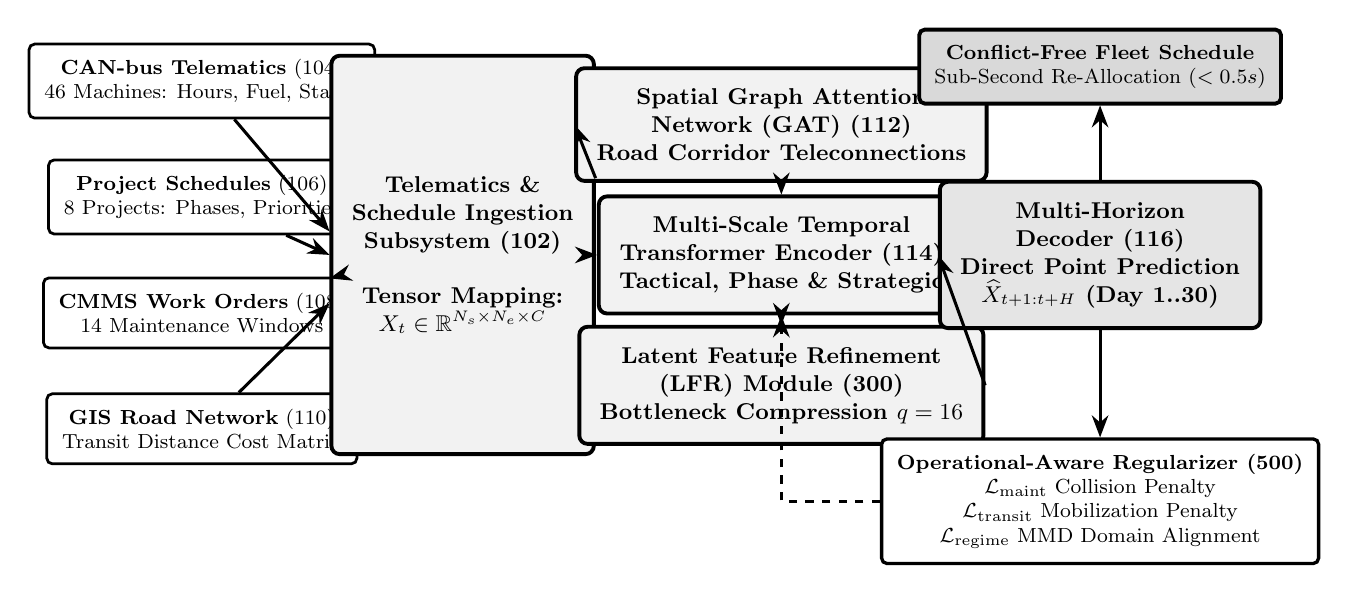
\begin{tikzpicture}[
    scale=0.92, every node/.style={transform shape},
    box/.style={draw=black, line width=1pt, rounded corners=2pt, align=center, fill=white, inner sep=6pt, font=\footnotesize},
    mainbox/.style={draw=black, line width=1.4pt, rounded corners=3pt, align=center, fill=gray!10, inner sep=8pt, font=\small\bfseries},
    arrow/.style={-Stealth, line width=1.1pt}
]
    % Inputs
    \node[box] (tele) at (-4.8, 4.0) {\textbf{CAN-bus Telematics} (104)\\46 Machines: Hours, Fuel, Status};
    \node[box] (sched) at (-4.8, 2.4) {\textbf{Project Schedules} (106)\\8 Projects: Phases, Priorities};
    \node[box] (cmms) at (-4.8, 0.8) {\textbf{CMMS Work Orders} (108)\\14 Maintenance Windows};
    \node[box] (gis) at (-4.8, -0.8) {\textbf{GIS Road Network} (110)\\Transit Distance Cost Matrix};

    % Ingestion
    \node[mainbox, minimum width=2.8cm, minimum height=5.5cm] (ingest) at (-1.2, 1.6) {\textbf{Telematics \&}\\\textbf{Schedule Ingestion}\\\textbf{Subsystem (102)}\\[1em] Tensor Mapping:\\$X_t \in \mathbb{R}^{N_s \times N_e \times C}$};

    % Core Modules
    \node[mainbox, minimum width=3.8cm] (gat) at (3.2, 3.4) {\textbf{Spatial Graph Attention}\\\textbf{Network (GAT) (112)}\\Road Corridor Teleconnections};
    \node[mainbox, minimum width=3.8cm] (trans) at (3.2, 1.6) {\textbf{Multi-Scale Temporal}\\\textbf{Transformer Encoder (114)}\\Tactical, Phase \& Strategic};
    \node[mainbox, minimum width=3.8cm] (lfr) at (3.2, -0.2) {\textbf{Latent Feature Refinement}\\\textbf{(LFR) Module (300)}\\Bottleneck Compression $q=16$};

    % Decoder
    \node[mainbox, minimum width=3.2cm, fill=gray!20] (dec) at (7.6, 1.6) {\textbf{Multi-Horizon}\\\textbf{Decoder (116)}\\Direct Point Prediction\\$\widehat{X}_{t+1:t+H}$ (Day 1..30)};

    % Regularizer
    \node[box, line width=1.2pt] (reg) at (7.6, -1.8) {\textbf{Operational-Aware Regularizer (500)}\\$\mathcal{L}_{\text{maint}}$ Collision Penalty\\$\mathcal{L}_{\text{transit}}$ Mobilization Penalty\\$\mathcal{L}_{\text{regime}}$ MMD Domain Alignment};

    % Output
    \node[box, line width=1.4pt, fill=gray!30] (out) at (7.6, 4.2) {\textbf{Conflict-Free Fleet Schedule}\\Sub-Second Re-Allocation ($<0.5s$)};

    % Connections
    \draw[arrow] (tele) -- (ingest.170);
    \draw[arrow] (sched) -- (ingest.180);
    \draw[arrow] (cmms) -- (ingest.190);
    \draw[arrow] (gis) -- (ingest.200);

    \draw[arrow] (ingest.30) -- (gat.west);
    \draw[arrow] (ingest.0) -- (trans.west);
    \draw[arrow] (gat) -- (trans);
    \draw[arrow] (trans) -- (lfr);
    \draw[arrow] (lfr.east) -- (dec.west);
    \draw[arrow] (dec.south) -- (reg.north);
    \draw[arrow] (dec.north) -- (out.south);
    \draw[arrow, dashed] (reg.west) -| (trans.south);

\end{tikzpicture}
\caption*{\textbf{FIG. 1:} OVERALL SYSTEM ARCHITECTURE BLOCK DIAGRAM OF CONSTRUMINDNET (100)}
\end{figure}

\newpage

% --- FIG. 2 & FIG. 3 ---
\begin{figure}[!ht]
\centering
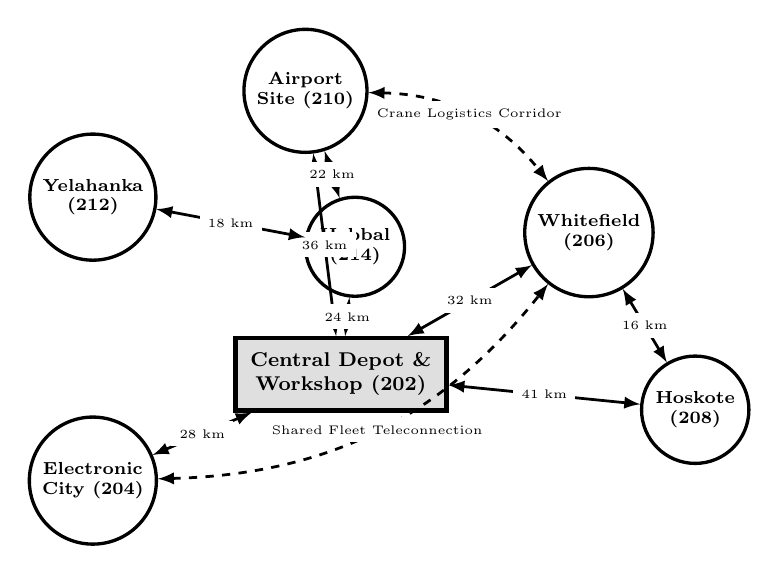
\begin{tikzpicture}[
    scale=0.9, every node/.style={transform shape},
    site/.style={circle, draw=black, line width=1.2pt, fill=white, inner sep=3pt, font=\scriptsize\bfseries, align=center},
    depot/.style={rectangle, draw=black, line width=1.6pt, fill=gray!25, inner sep=6pt, font=\footnotesize\bfseries, align=center},
    road/.style={latex-latex, line width=1pt}
]
    % Spatial Nodes
    \node[depot] (D) at (0, 0) {Central Depot \&\\Workshop (202)};
    \node[site] (EC) at (-3.5, -1.5) {Electronic\\City (204)};
    \node[site] (WF) at (3.5, 2.0) {Whitefield\\(206)};
    \node[site] (HK) at (5.0, -0.5) {Hoskote\\(208)};
    \node[site] (AP) at (-0.5, 4.0) {Airport\\Site (210)};
    \node[site] (YL) at (-3.5, 2.5) {Yelahanka\\(212)};
    \node[site] (HB) at (0.2, 1.8) {Hebbal\\(214)};

    % Roads
    \draw[road] (D) -- node[fill=white, font=\tiny] {28 km} (EC);
    \draw[road] (D) -- node[fill=white, font=\tiny] {32 km} (WF);
    \draw[road] (D) -- node[fill=white, font=\tiny] {41 km} (HK);
    \draw[road] (D) -- node[fill=white, font=\tiny] {36 km} (AP);
    \draw[road] (D) -- node[fill=white, font=\tiny] {24 km} (HB);
    \draw[road] (HB) -- node[fill=white, font=\tiny] {18 km} (YL);
    \draw[road] (HB) -- node[fill=white, font=\tiny] {22 km} (AP);
    \draw[road] (WF) -- node[fill=white, font=\tiny] {16 km} (HK);
    \draw[road, dashed] (EC) to[bend right=25] node[fill=white, font=\tiny] {Shared Fleet Teleconnection} (WF);
    \draw[road, dashed] (AP) to[bend left=25] node[fill=white, font=\tiny] {Crane Logistics Corridor} (WF);

\end{tikzpicture}
\caption*{\textbf{FIG. 2:} NON-EUCLIDEAN SPATIO-TEMPORAL LOGISTICS GRAPH NETWORK (200)}
\end{figure}

\vspace{2em}

\begin{figure}[!ht]
\centering
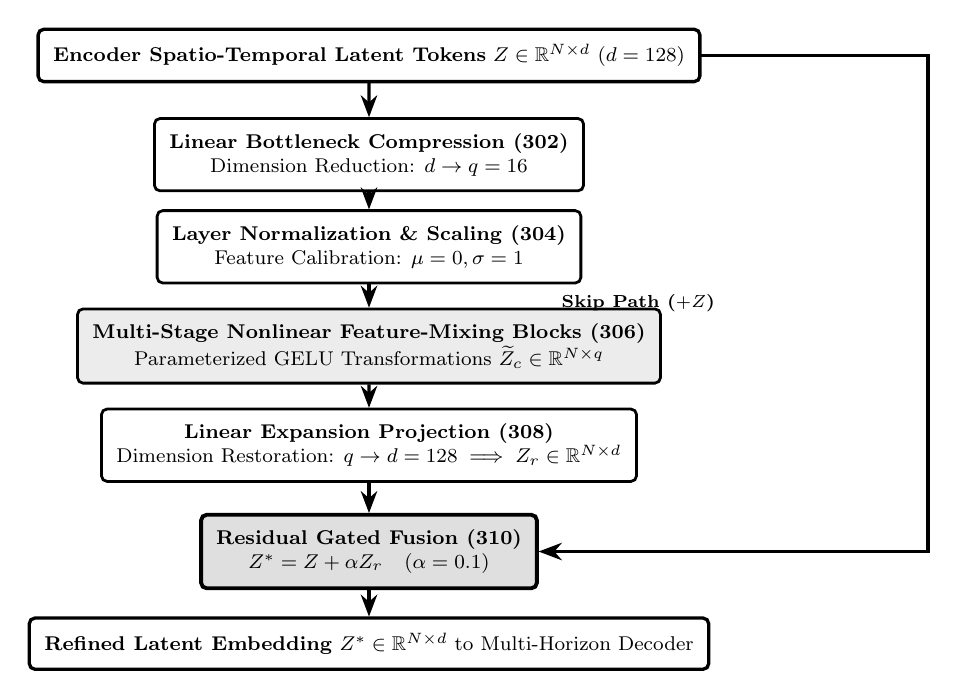
\begin{tikzpicture}[
    scale=0.9, every node/.style={transform shape},
    box/.style={draw=black, line width=1pt, rounded corners=2pt, align=center, fill=white, inner sep=6pt, font=\footnotesize},
    arrow/.style={-Stealth, line width=1.1pt}
]
    \node[box, line width=1.2pt] (in) at (0, 4.2) {\textbf{Encoder Spatio-Temporal Latent Tokens} $Z \in \mathbb{R}^{N \times d}$ ($d = 128$)};
    \node[box] (comp) at (0, 2.8) {\textbf{Linear Bottleneck Compression (302)}\\Dimension Reduction: $d \to q = 16$};
    \node[box] (norm) at (0, 1.5) {\textbf{Layer Normalization \& Scaling (304)}\\Feature Calibration: $\mu=0, \sigma=1$};
    \node[box, fill=gray!15] (mix) at (0, 0.1) {\textbf{Multi-Stage Nonlinear Feature-Mixing Blocks (306)}\\Parameterized GELU Transformations $\widetilde{Z}_c \in \mathbb{R}^{N \times q}$};
    \node[box] (exp) at (0, -1.3) {\textbf{Linear Expansion Projection (308)}\\Dimension Restoration: $q \to d = 128 \implies Z_r \in \mathbb{R}^{N \times d}$};
    \node[box, line width=1.4pt, fill=gray!25] (fuse) at (0, -2.8) {\textbf{Residual Gated Fusion (310)}\\$Z^* = Z + \alpha Z_r \quad (\alpha = 0.1)$};
    \node[box, line width=1.2pt] (out) at (0, -4.1) {\textbf{Refined Latent Embedding} $Z^* \in \mathbb{R}^{N \times d}$ to Multi-Horizon Decoder};

    \draw[arrow] (in) -- (comp);
    \draw[arrow] (comp) -- (norm);
    \draw[arrow] (norm) -- (mix);
    \draw[arrow] (mix) -- (exp);
    \draw[arrow] (exp) -- (fuse);
    \draw[arrow] (fuse) -- (out);

    % Residual skip connection
    \draw[arrow, line width=1.2pt] (in.east) -- ++(3.2, 0) |- (fuse.east);
    \node[font=\scriptsize\bfseries] at (3.8, 0.7) {Skip Path ($+Z$)};

\end{tikzpicture}
\caption*{\textbf{FIG. 3:} LATENT FEATURE REFINEMENT (LFR) MODULE DETAIL (300)}
\end{figure}

\newpage

% --- FIG. 4 & FIG. 5 ---
\begin{figure}[!ht]
\centering
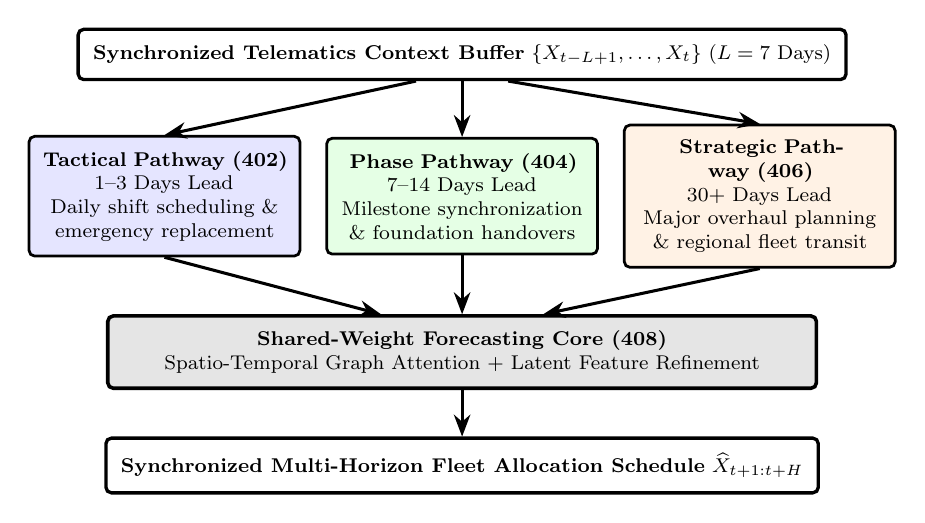
\begin{tikzpicture}[
    scale=0.9, every node/.style={transform shape},
    box/.style={draw=black, line width=1pt, rounded corners=2pt, align=center, fill=white, inner sep=6pt, font=\footnotesize},
    arrow/.style={-Stealth, line width=1.1pt}
]
    \node[box, line width=1.2pt, minimum width=10cm] (raw) at (0, 3.8) {\textbf{Synchronized Telematics Context Buffer} $\{X_{t-L+1}, \dots, X_t\}$ ($L = 7$ Days)};

    \node[box, fill=blue!10, text width=3.4cm] (tac) at (-4.2, 1.8) {\textbf{Tactical Pathway (402)}\\1--3 Days Lead\\Daily shift scheduling \& emergency replacement};
    \node[box, fill=green!10, text width=3.4cm] (ph) at (0, 1.8) {\textbf{Phase Pathway (404)}\\7--14 Days Lead\\Milestone synchronization \& foundation handovers};
    \node[box, fill=orange!10, text width=3.4cm] (strat) at (4.2, 1.8) {\textbf{Strategic Pathway (406)}\\30+ Days Lead\\Major overhaul planning \& regional fleet transit};

    \node[box, line width=1.3pt, fill=gray!20, minimum width=10cm] (core) at (0, -0.4) {\textbf{Shared-Weight Forecasting Core (408)}\\Spatio-Temporal Graph Attention + Latent Feature Refinement};

    \node[box, line width=1.2pt, minimum width=10cm] (out) at (0, -2.0) {\textbf{Synchronized Multi-Horizon Fleet Allocation Schedule} $\widehat{X}_{t+1:t+H}$};

    \draw[arrow] (raw.210) -- (tac.north);
    \draw[arrow] (raw.south) -- (ph.north);
    \draw[arrow] (raw.330) -- (strat.north);

    \draw[arrow] (tac.south) -- (core.155);
    \draw[arrow] (ph.south) -- (core.north);
    \draw[arrow] (strat.south) -- (core.25);

    \draw[arrow] (core) -- (out);

\end{tikzpicture}
\caption*{\textbf{FIG. 4:} MULTI-SCALE TEMPORAL DECOMPOSITION HIERARCHY (400)}
\end{figure}

\vspace{1.5em}

\begin{figure}[!ht]
\centering
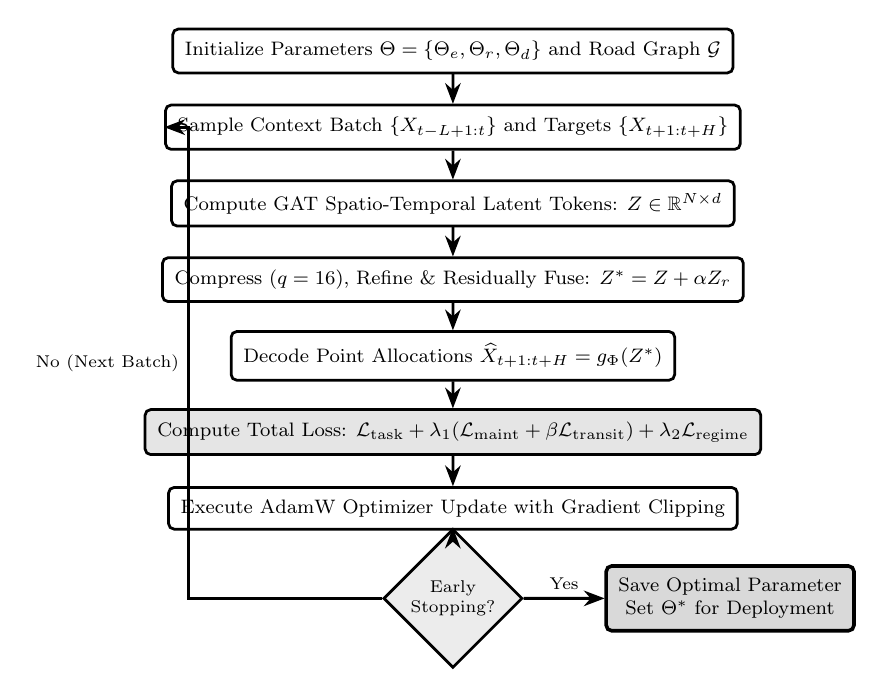
\begin{tikzpicture}[
    scale=0.88, every node/.style={transform shape},
    stepbox/.style={draw=black, line width=1pt, rounded corners=2pt, align=center, fill=white, inner sep=5pt, font=\footnotesize},
    decision/.style={diamond, draw=black, line width=1pt, align=center, fill=gray!15, inner sep=2pt, font=\scriptsize},
    arrow/.style={-Stealth, line width=1pt}
]
    \node[stepbox] (s1) at (0, 4.5) {Initialize Parameters $\Theta = \{\Theta_e, \Theta_r, \Theta_d\}$ and Road Graph $\mathcal{G}$};
    \node[stepbox] (s2) at (0, 3.4) {Sample Context Batch $\{X_{t-L+1:t}\}$ and Targets $\{X_{t+1:t+H}\}$};
    \node[stepbox] (s3) at (0, 2.3) {Compute GAT Spatio-Temporal Latent Tokens: $Z \in \mathbb{R}^{N \times d}$};
    \node[stepbox] (s4) at (0, 1.2) {Compress ($q=16$), Refine \& Residually Fuse: $Z^* = Z + \alpha Z_r$};
    \node[stepbox] (s5) at (0, 0.1) {Decode Point Allocations $\widehat{X}_{t+1:t+H} = g_\Phi(Z^*)$};
    \node[stepbox, fill=gray!20] (s6) at (0, -1.0) {Compute Total Loss: $\mathcal{L}_{\text{task}} + \lambda_1 (\mathcal{L}_{\text{maint}} + \beta \mathcal{L}_{\text{transit}}) + \lambda_2 \mathcal{L}_{\text{regime}}$};
    \node[stepbox] (s7) at (0, -2.1) {Execute AdamW Optimizer Update with Gradient Clipping};
    \node[decision] (s8) at (0, -3.4) {Early\\Stopping?};
    \node[stepbox, line width=1.3pt, fill=gray!30] (s9) at (4.0, -3.4) {Save Optimal Parameter\\Set $\Theta^*$ for Deployment};

    \draw[arrow] (s1) -- (s2);
    \draw[arrow] (s2) -- (s3);
    \draw[arrow] (s3) -- (s4);
    \draw[arrow] (s4) -- (s5);
    \draw[arrow] (s5) -- (s6);
    \draw[arrow] (s6) -- (s7);
    \draw[arrow] (s7) -- (s8);
    \draw[arrow] (s8) -- node[above, font=\scriptsize] {Yes} (s9);
    \draw[arrow] (s8.west) -- ++(-2.8,0) |- node[near start, left, font=\scriptsize] {No (Next Batch)} (s2.west);

\end{tikzpicture}
\caption*{\textbf{FIG. 5:} FLOWCHART OF END-TO-END MODEL TRAINING PROCEDURE (500)}
\end{figure}

\newpage

% --- FIG. 6 ---
\begin{figure}[!ht]
\centering
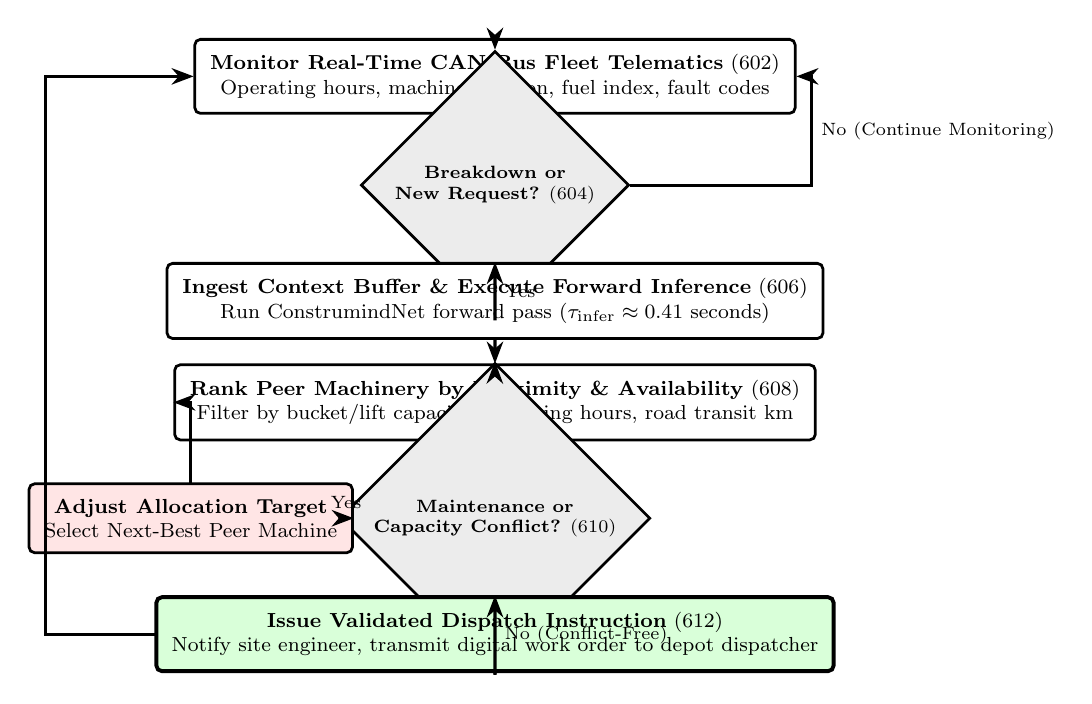
\begin{tikzpicture}[
    scale=0.92, every node/.style={transform shape},
    stepbox/.style={draw=black, line width=1pt, rounded corners=2pt, align=center, fill=white, inner sep=6pt, font=\footnotesize},
    decision/.style={diamond, draw=black, line width=1pt, align=center, fill=gray!15, inner sep=3pt, font=\scriptsize},
    arrow/.style={-Stealth, line width=1.1pt}
]
    \node[stepbox] (r1) at (0, 4.5) {\textbf{Monitor Real-Time CAN-Bus Fleet Telematics} (602)\\Operating hours, machine position, fuel index, fault codes};

    \node[decision] (r2) at (0, 3.0) {\textbf{Breakdown or}\\ \textbf{New Request?} (604)};

    \node[stepbox] (r3) at (0, 1.4) {\textbf{Ingest Context Buffer \& Execute Forward Inference} (606)\\Run ConstrumindNet forward pass ($\tau_{\text{infer}} \approx 0.41$ seconds)};

    \node[stepbox] (r4) at (0, 0.0) {\textbf{Rank Peer Machinery by Proximity \& Availability} (608)\\Filter by bucket/lift capacity, operating hours, road transit km};

    \node[decision] (r5) at (0, -1.6) {\textbf{Maintenance or}\\ \textbf{Capacity Conflict?} (610)};

    \node[stepbox, fill=red!10] (r6) at (-4.2, -1.6) {\textbf{Adjust Allocation Target}\\Select Next-Best Peer Machine};

    \node[stepbox, line width=1.4pt, fill=green!15] (r7) at (0, -3.2) {\textbf{Issue Validated Dispatch Instruction} (612)\\Notify site engineer, transmit digital work order to depot dispatcher};

    \draw[arrow] (r1) -- (r2);
    \draw[arrow] (r2) -- node[right, font=\scriptsize] {Yes} (r3);
    \draw[arrow] (r2.east) -- ++(2.5,0) |- node[near start, right, font=\scriptsize] {No (Continue Monitoring)} (r1.east);
    \draw[arrow] (r3) -- (r4);
    \draw[arrow] (r4) -- (r5);
    \draw[arrow] (r5) -- node[above, font=\scriptsize] {Yes} (r6);
    \draw[arrow] (r6) |- (r4);
    \draw[arrow] (r5) -- node[right, font=\scriptsize] {No (Conflict-Free)} (r7);
    \draw[arrow] (r7.west) -- ++(-1.5,0) |- (r1.west);

\end{tikzpicture}
\caption*{\textbf{FIG. 6:} REAL-TIME ROLLOUT, CONFLICT DETECTION, AND SUB-SECOND DISPATCHING (600)}
\end{figure}

\label{LastPage}

\end{document}
